\subsection{Workshop: Medical Imaging Meets NeurIPS}

\subsubsection{DeepSim: Semantic similarity metrics for learned image registration \cite{abs-2011-05735}}

Presented by \textit{Steffen Czolbe}. \\

{\bf Motivation:} having a decent solution of image registration as an ill-posed problem is heavily dependent on the presence of a meaningful distance metric $D$ (fig. \ref{fig:image_reg_problem_setting}). \\

\begin{figure}[!h]
    \centering
    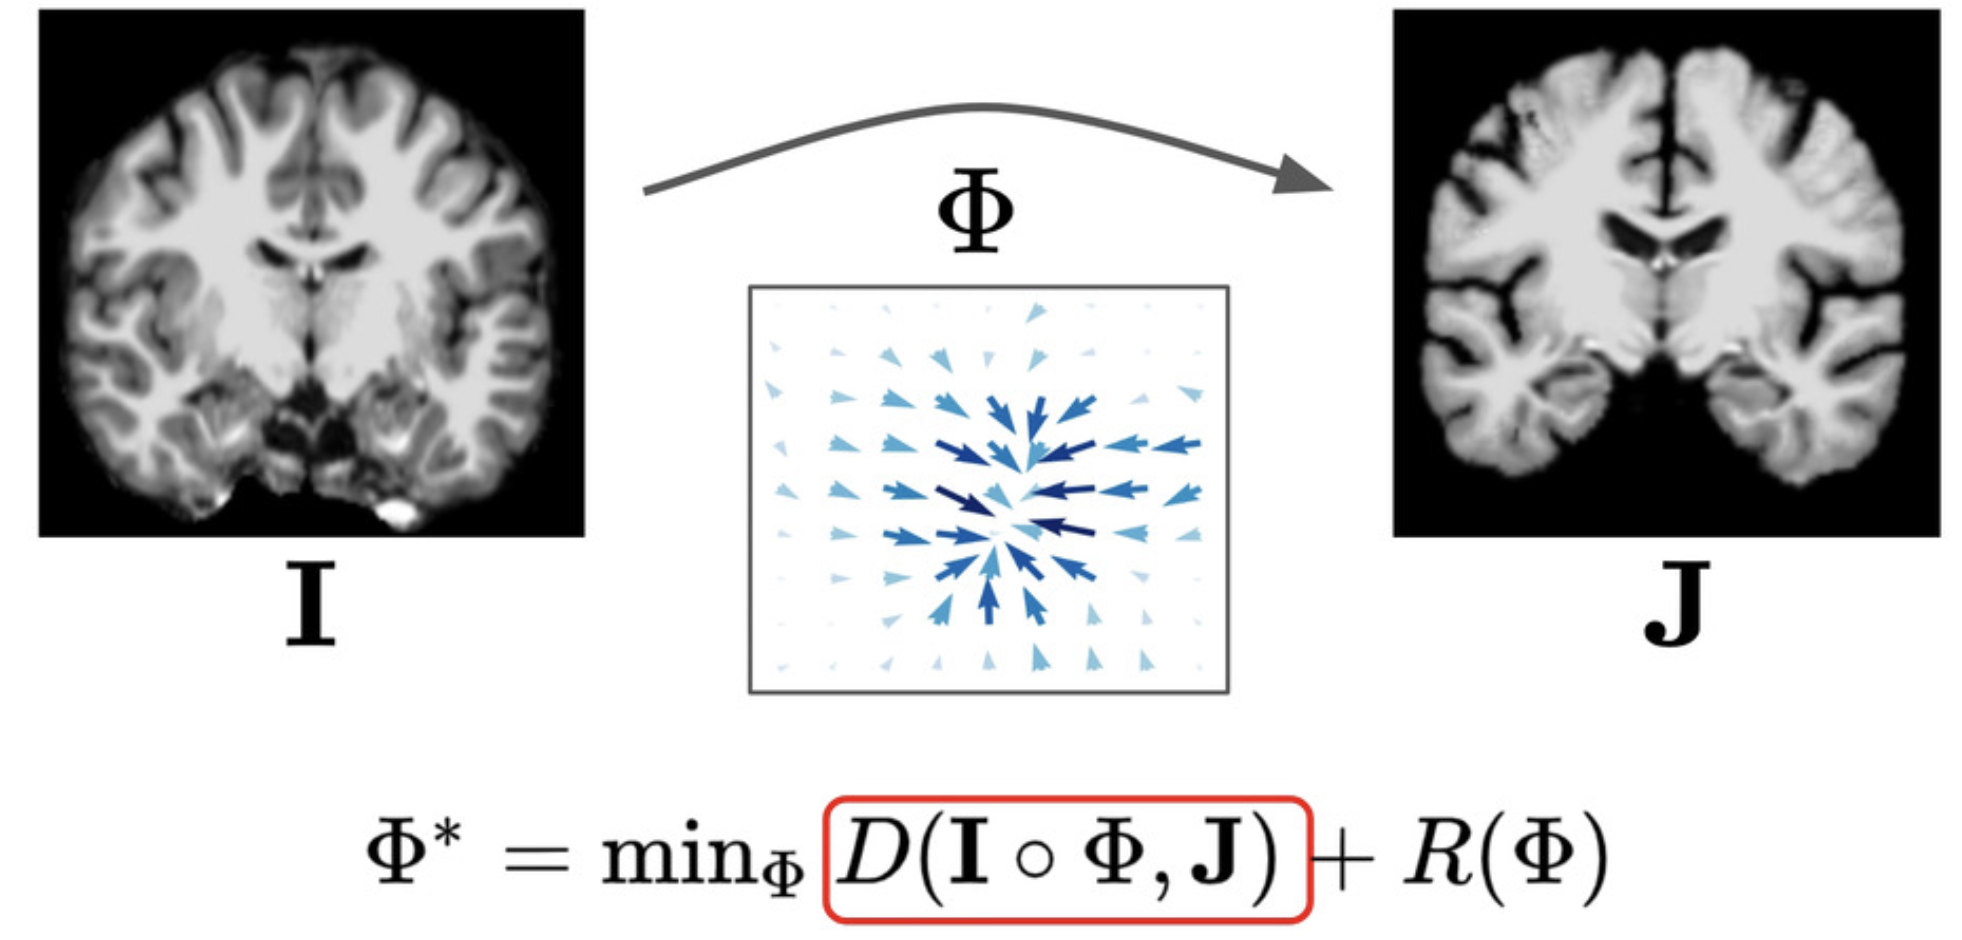
\includegraphics[scale=0.4]{neurips-2020/images/Screenshot 2020-12-15 at 16.48.59.png}
    \caption{Medical image registration problem setting. Selection of a distance metric $D$ plays a key role.}
    \label{fig:image_reg_problem_setting}
\end{figure}

{\bf Observation:} typically, the distance in image registration task is computed on patches as pixel-wise cosine distance (eq. \ref{eq:pixel_wise_cosine_distance}) between reconstruction and some generated reference.
The problem here is that pixel-wise esitmations are typically not very accurate and can be improved by replacing pixel with some more high-level features.

\begin{equation}
    NCC_{patch} (A, B) = \frac{<A - \hat{A}, B - \hat{B}>}{|| A - \hat{A} || || B - \hat{B} ||}
    \label{eq:pixel_wise_cosine_distance}
\end{equation}

{\bf Method:} pretrain some feature extractor on a proxy task withing the same imaging domain (segmentation), use its features as an enriched substitutions of raw pixel values (eq. \ref{eq:features_consine_distance}). 

\begin{equation}
    DeepSim_{patch} (A, B) = \frac{< F(A), F(B) >}{|| F(A) || || F(B) ||}
    \label{eq:features_consine_distance}
\end{equation}

{\bf Results:} as claimed:
\begin{itemize}
    \item High registration accuracy across multiple datasets
    \item The metric is general and can be applied to different modalities and algorithms 
    \itema Translations results are smoother
\end{itemize}





\subsubsection{Using StyleGANs for Visual Interpretability of Deep Learning Models on Medical Images \href{http://www.cse.cuhk.edu.hk/~qdou/public/medneurips2020/70_neurips2020_cameraready_opt.pdf}{paper}}

Presented by \textit{Kathryn Schutte}. \\

{\bf Motivation:} intractability of Machine Learning models in important, especially in medical imaging. 
The goal is to improve intractability by proposing an alternative go the currently popular GradCAM \cite{SelvarajuCDVPB17} approach. \\

{\bf Observation:} currently used methods (for example GradCAM) only highlight regions of an image that has the highest contribution to the result that a model outputs.
Instead, one could generate an image view that would lead to another output. Example is shown on the fig. \ref{fig:gradual_changes}. \\

\begin{figure}[h!]
    \centering
    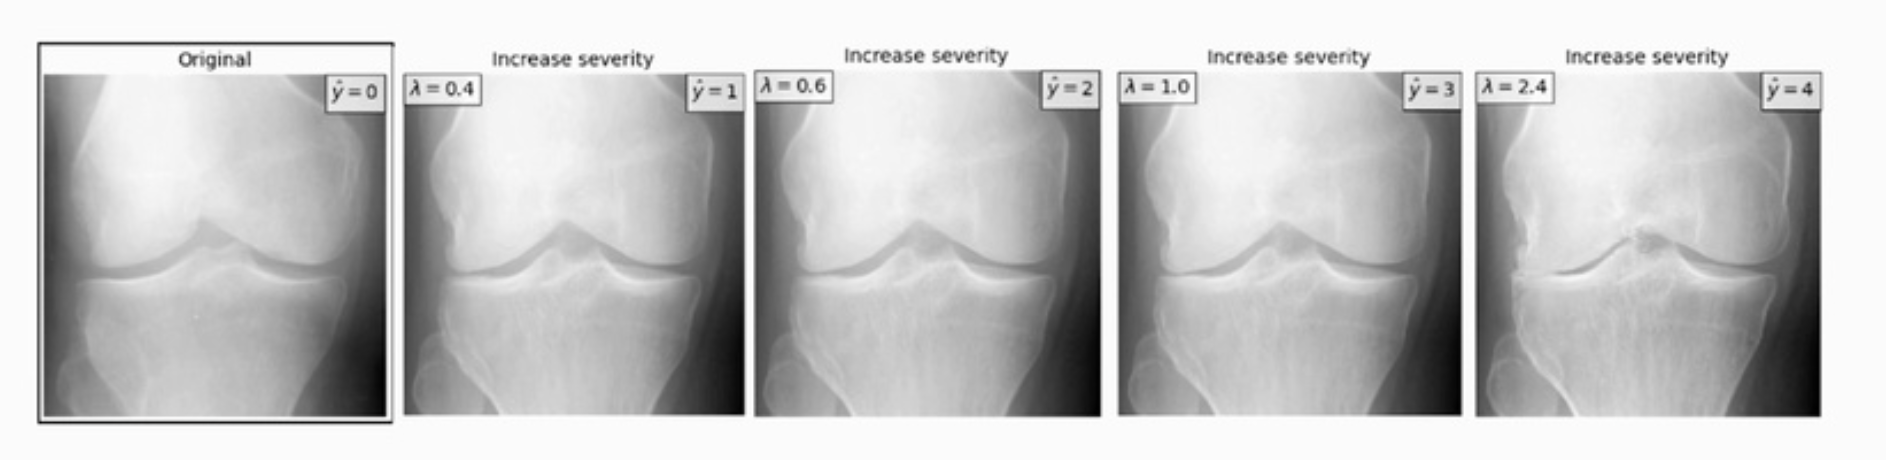
\includegraphics[scale=0.4]{neurips-2020/images/Screenshot 2020-12-15 at 20.22.51.png}
    \caption{Illustration changes of image view that could lead to a different model output. In this case classification task is considered and the initial output of the model is 0 (no pathology). However, one can have a hard time understanding why the prediction is so. For that, the proposed method generates transformations of the initial image that would lead to the alternative classification results.}
    \label{fig:gradual_changes}
\end{figure}

{\bf Method:} the following pipeline is proposed:

{\bf Step 1:} train a StyleGAN model \cite{KarrasLA19}. StyleGAN is chosen because 1) it is able to generate high-quality images and 2) has an interpretable latent space vector in the bottleneck of the generator, which can be used to generate images with desired qualities (check out StyleGAN paper for more information).

{\bf Step 2:} find the direction, which has the greatest impact on the model's output (in the particular case - on Osteoarthritis severity).

\begin{equation}
    \tilde{f} (w) = \sigma (\alpha^T \textbf{w} + \beta) \approx f(g(w))
\end{equation}

So if we approximate classifier fitting a logistic regression $f$ to this latent space we can retrieve the direction of Osteoarthritis severity using $\alpha$. 
It means, that on this stage we first build a labeled dataset of latent vectors (otherwise they are hard to interpret).

{\bf Step 3:} Encode the real images into the latent space (fig. \ref{fig:encoding_of_real_images}). \\

\begin{figure}[h!]
    \centering
    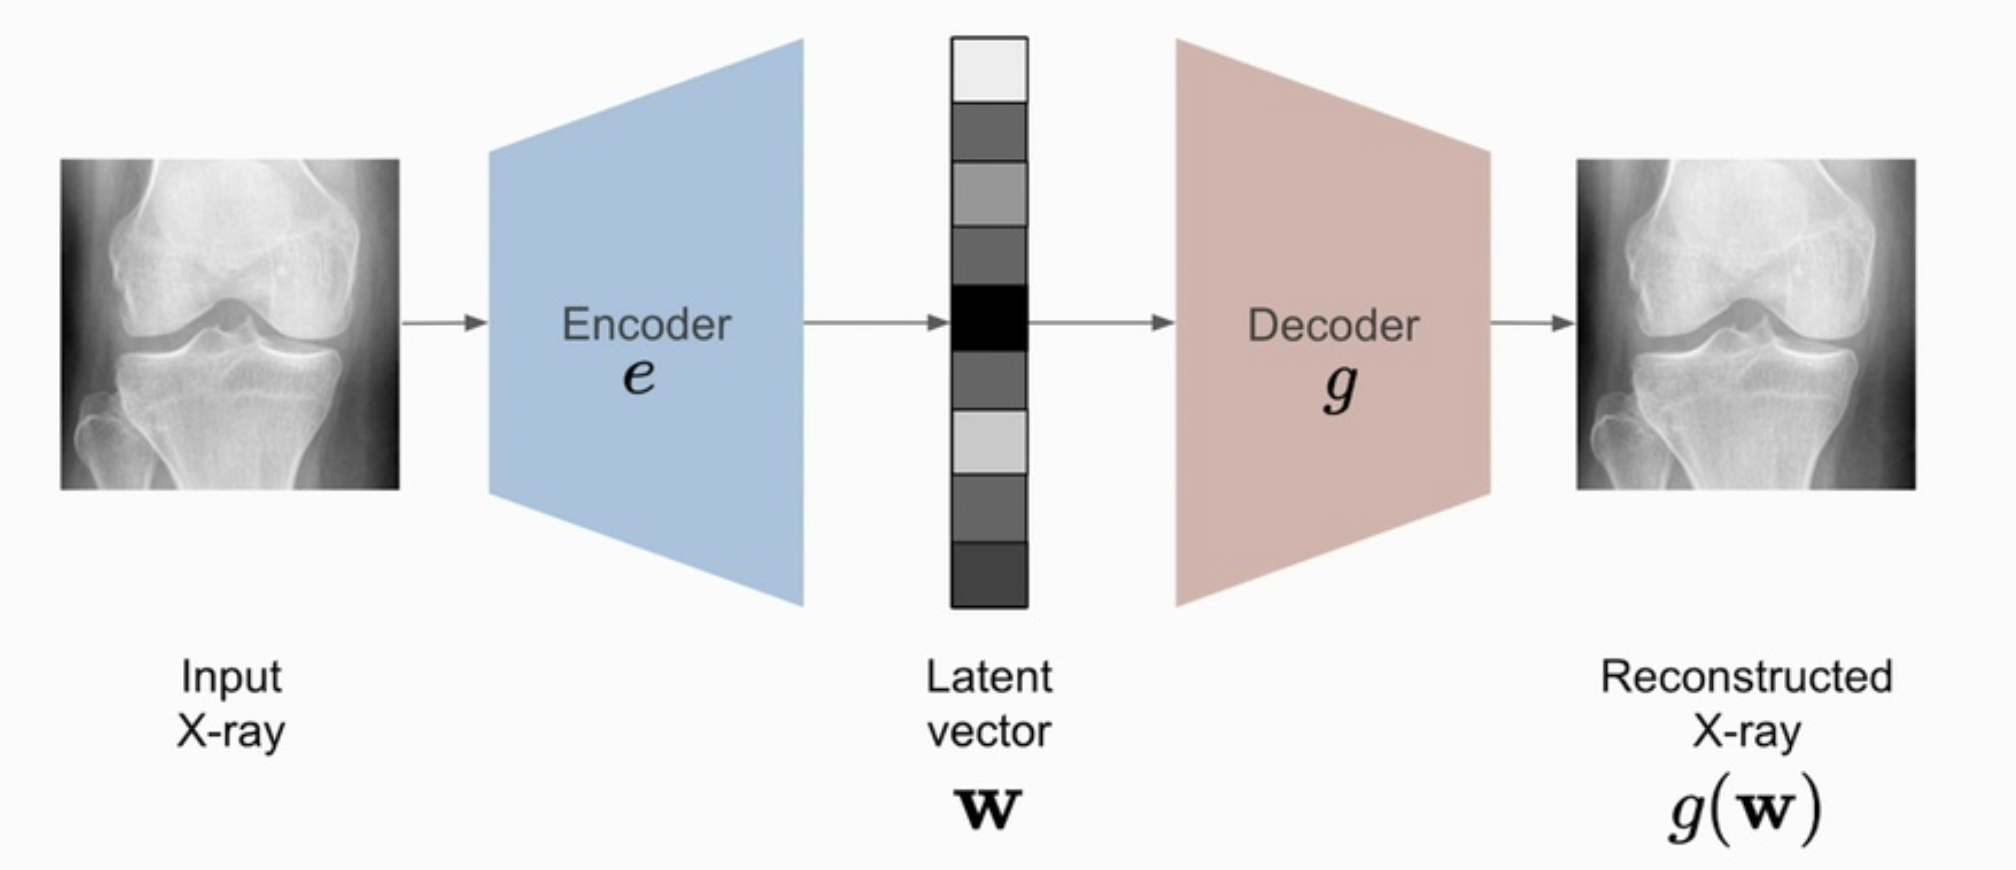
\includegraphics[scale=0.4]{neurips-2020/images/Screenshot 2020-12-15 at 20.39.44.png}
    \caption{The last step of the proposed pipeline - encoding real images into latent vectors.}
    \label{fig:encoding_of_real_images}
\end{figure}

{\bf Results:} generated images seem to be reasonable, however the solution still looks very task-specific. 
Not clear whether the proposed method will give reliable results on other domains, especially considering the fact that GAN training is in general data-hungry and available datasets may not be enough.
Also not clear how to transfer the approach for the regression task (if it is possible at all).






\subsubsection{FastMRI keynote: Fast(er) MRI: a radiologist's perspective}

Presented by \textit{Yvonne Lui}. \\

{\bf Motivation:} discuss results of this year's challenge, compare them with the ones from the previous year. \\

{\bf Observation:} organizers claim that overall SSIM has a decent correlation with radiologist's rankings of challenge results. 
More concretely, when SSIM values are very different, their relative order well correlates with the order provided my manual evaluations with radiologists.
However, when differences in values are small (3rd-4th digit), like we can commonly observe in top-3 of the leaderboard, relative order may be different. 
In particular, top-2 and top-3 results (according to their SSIM scores, difference in the 3rd digit) were flipped after evaluation from radiologists. \\

{\bf Observation:} top-3 values of SSIM scores from 2020 challenge are much higher than corresponding values from the previous year.
2019 winner would not get into top-3 in 2020 with the same SSIM score. 
However, it is not clear whether such a direct comparison is fair due to the fact that 2019 and 2020 challenges utilized very different data (different anatomies, protocols). \\

{\bf Observation:} last year's manual evaluation procedure was not aimed at finding the most accurate (from the anatomical perspective) reconstructions.
Instead, radiologists only judged on the perceptual feeling of quality, which led to the problem illustrated on fig. \ref{fig:2019_problems}. 
Here, none of the reconstructions was good enough to capture the important anatomical structure while radiologists ranked all these reconstructions to be high-quality. \\

\begin{figure}[h!]
    \centering
    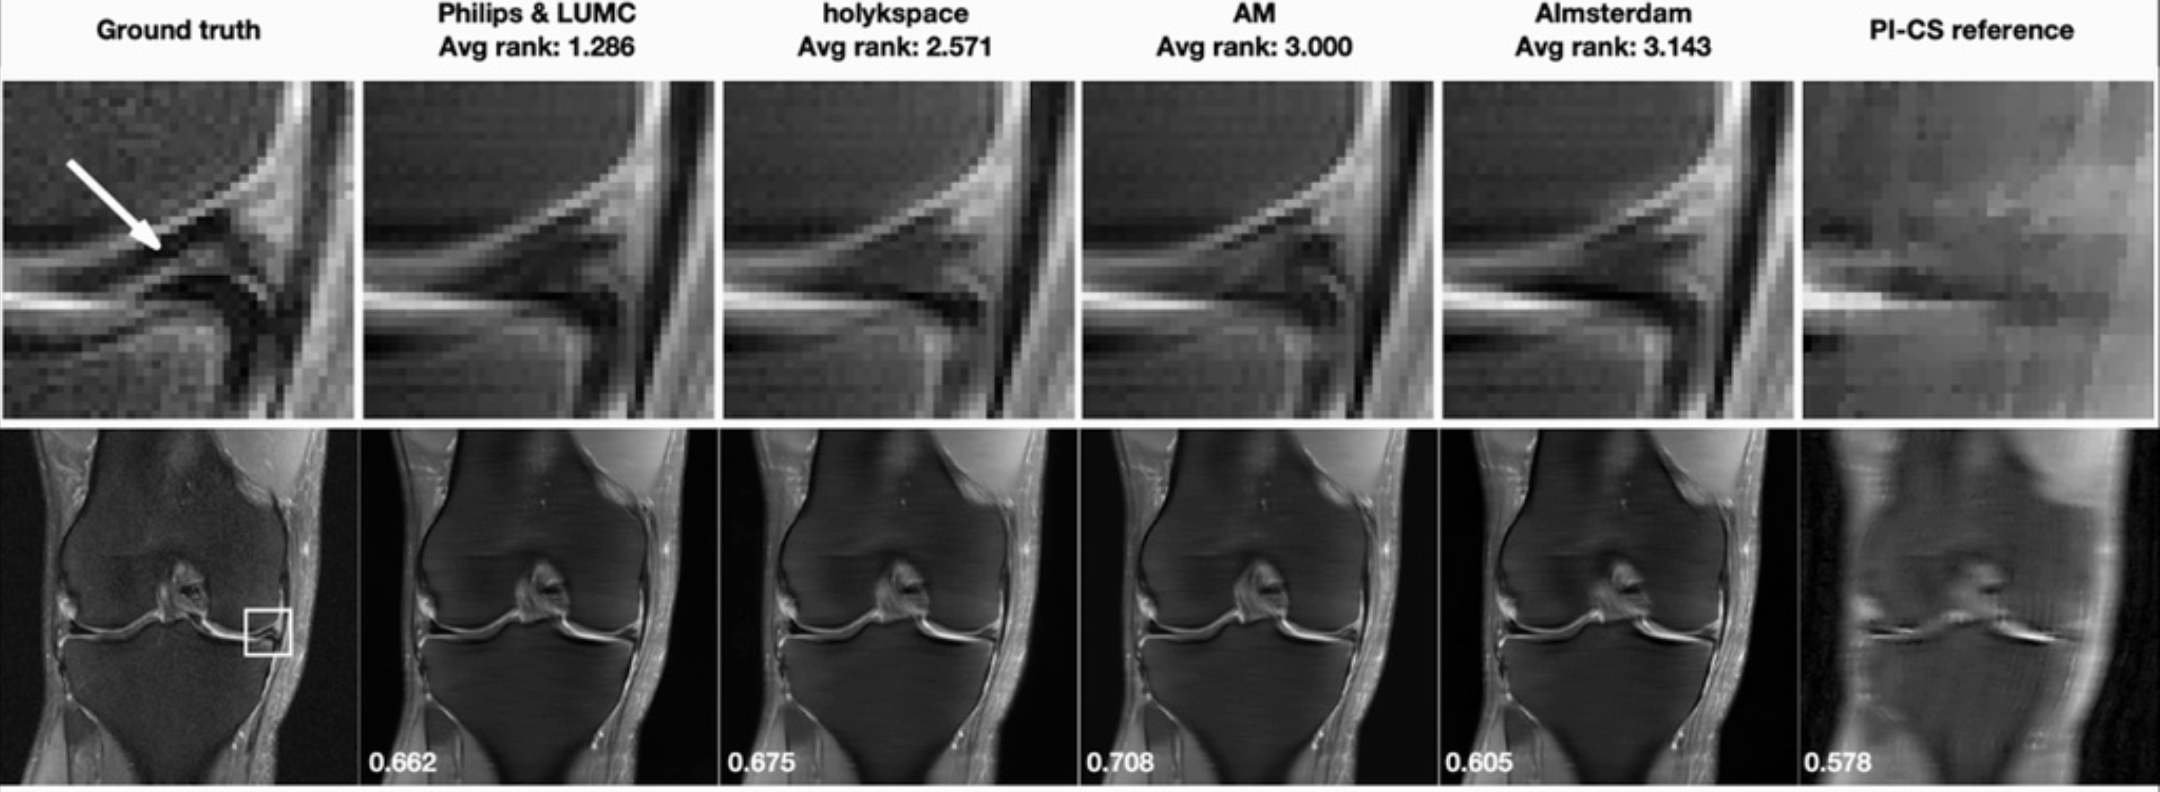
\includegraphics[scale=0.4]{neurips-2020/images/Screenshot 2020-12-15 at 11.17.48.png}
    \caption{Example from the 2019 challenge, when all reconstructions failed to preserve an important anatomical structures but still were hightly ranked by experts.}
    \label{fig:2019_problems}
\end{figure}

To avoid the same problem this year, organizers revised the evaluation process and carefully selected several pathologies. \\

{\bf New evaluation process:} radiologist were asked to rank reconstructions by assigning them scores from 1 to 4, where lower is better in for different criteria: presence of artefacts, sharpness and contrast-to-noise ratio (CNR). \\

{\bf Multi-coil 4x and 8x tracks:} this is very similar challenge to the 2019 version except from data and the evaluation process. 
The presentation of results of showed that 8x acceleration is still to high for a potential clinical application with diagnostic purposes. \\

{\bf Transfer track:} this track was aimed to estimate how good model trained on data from one vendor can be used on data from another vendors.
In particular Siemens data was used for training and transferring was tested on GE and Philips data.
Overall, Philips appeared to be closer to Siemens data resulting in (in general) better reconstructions. 
However, results greatly vary depending on contrast and particular anatomical structures.

{\bf Note:} one of competitors this year also provided estimates of coil sensitivity maps (CSMs) as a part of their submission.
This could help them to increase the overall quality (not clear whether it helped a lot though).

{\bf Note:} presented mentioned the work from MRM (early 2020) on Gibbs deringing \cite{Muckley_2020} where authors were able to create a system for Gibbs ringing removing. The artefacts were result of a partial Fourier transform.
They did it by training a neural network on ImageNet dataset for the deringing task. 
Then this model was applied to MRI data and showed a decent performance. \\



